\clearpage
\subsection{Ultrasonic evaluation}
As already stated we have measured the intensity distribution of the laser
passing through a phase grating, in particular the phase grating created
by ultrasonic waves passing through the medium. We evaluate these diffraction patterns
by determining the position of the maxima and their intensities with an algorithm
by extremal analysis. The results are seen in 
figure~\ref{fig:ultrasonic1}.
The error of this analysis
is given by the width of the respective peaks, the error on the amplitude is 
taken to be the error if the oscilloscope, as described before \eqref{eq:error_osci}.
The conversion from time to angle was given in the previous section (see
figure\ref{fig:calibrate_fit} for the conversion fit). In the following we 
will give all information in the captions of the figures and tables, respectively.
We will give the least square fits for the maxima from order zero to three and 
their coefficients along with the covariance matrices.

\begin{figure}[H]
    \centering
    \begin{subfigure}[b]{\picwidth}
        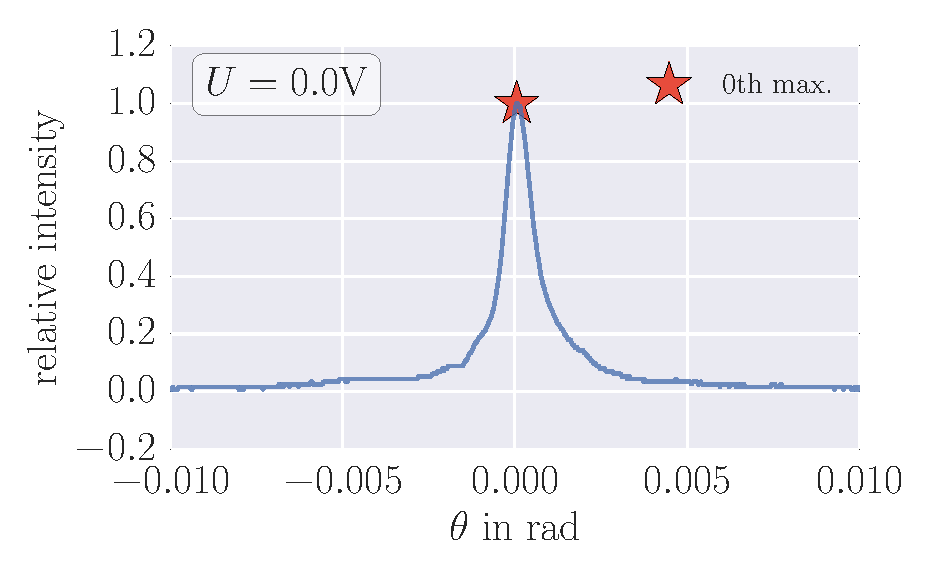
\includegraphics[width=1.0\textwidth]{analysis/figures/raman_001}
        \caption{}
        \label{fig:raman_001}
    \end{subfigure}
    \begin{subfigure}[b]{\picwidth}
        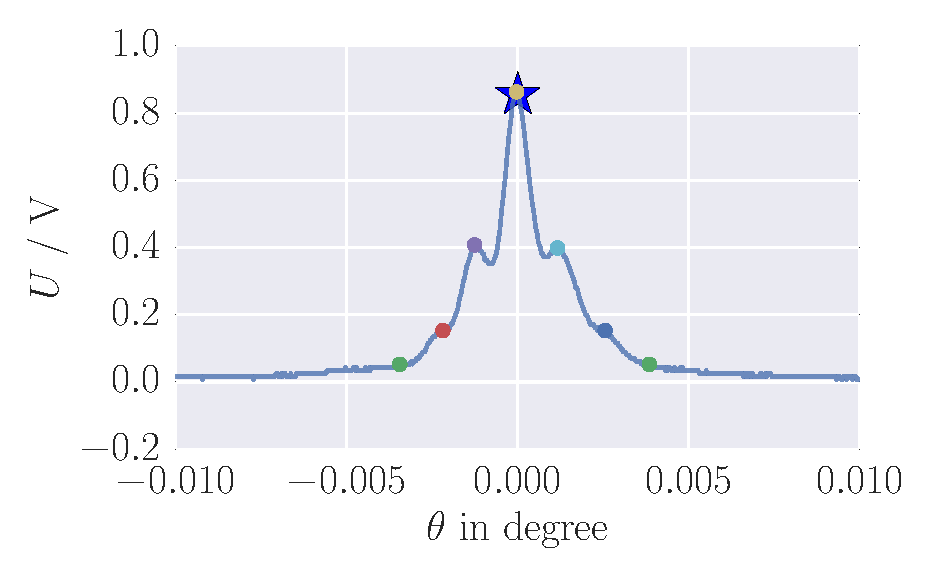
\includegraphics[width=1.0\textwidth]{analysis/figures/raman_007}
        \caption{}
        \label{fig:raman_007}
    \end{subfigure}
    \begin{subfigure}[b]{\picwidth}
        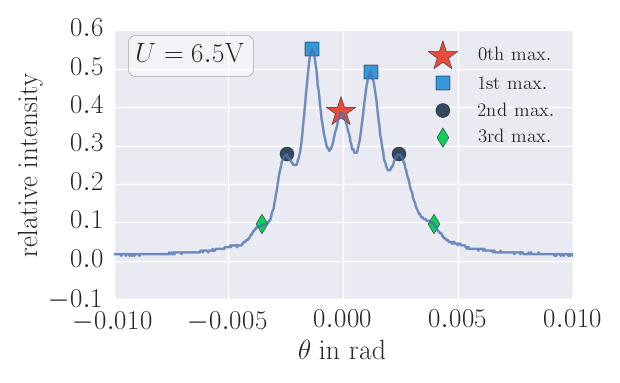
\includegraphics[width=1.0\textwidth]{analysis/figures/raman_014}
        \caption{}
        \label{fig:raman_014}
    \end{subfigure}
    \begin{subfigure}[b]{\picwidth}
        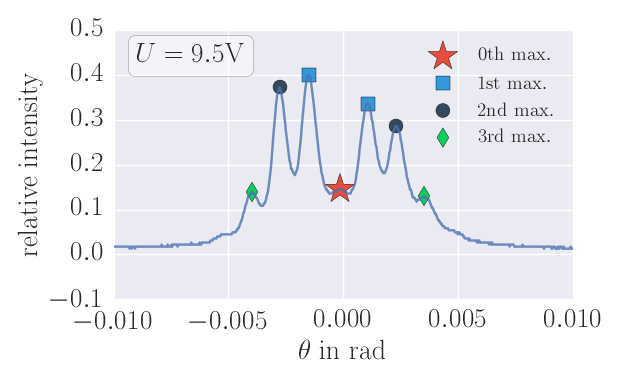
\includegraphics[width=1.0\textwidth]{analysis/figures/raman_020}
        \caption{}
        \label{fig:raman_020}
    \end{subfigure}
    \caption{
        These figures constitute a selection of the available measurements 
        from the ultrasonic experiment. We denoted the 
        different orders by different symbols (see the respective legends). 
        The maxima were estimated by an algorithm which seeks for local extrema
        and evaluates them with a certain threshold. The threshold is determined 
        by the minimal distance of maxima, estimated by the theoretical 
        relationship $sin(\theta) = m \lambda / \Lambda$. 
        The intensities are given by the measured voltage,
        normed by the zeroth maximum at $U=0V$.
        }
    \label{fig:ultrasonic1}
\end{figure}
\newpage
\begin{figure}
    \centering
    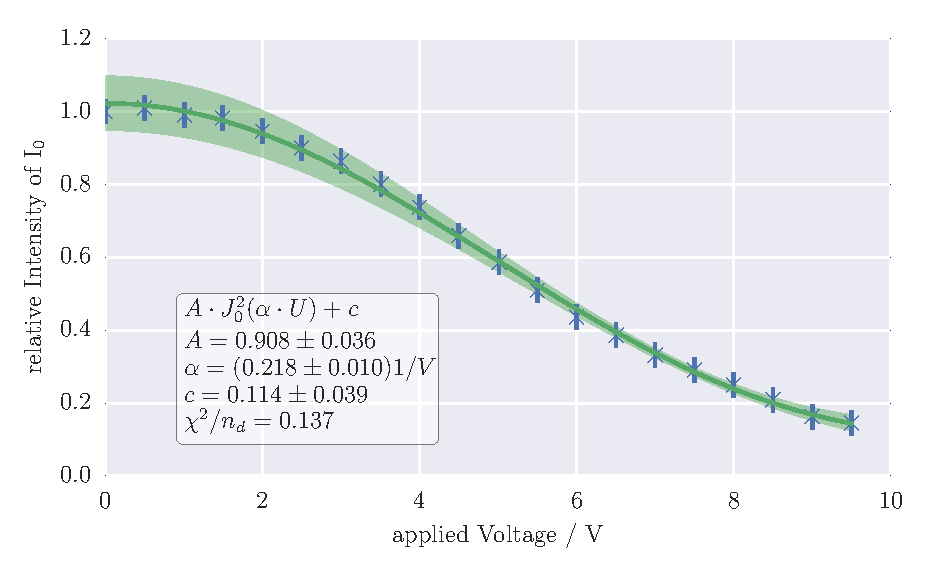
\includegraphics[width=1\textwidth]{analysis/figures/besselfit_000}
    \caption{The measurements and the least square fit with the maxima of order zero. 
    The error bars are given by 3\% of the extent of the oscilloscope,
    while the light green surface is the upper and lower limit of the fitted function, calculated 
    with the covariance matrix of the coefficients. 
    We fit the data with the function derived in the theoretical
    section, but extent it by an factor $c$ in order to take into account an additional (constant) noise
    influencing the photo diodes. 
    \\
    $\Rightarrow$ We notice the agreement of our measurements with the Raman-Nath theory. Using the
    coefficient $\alpha$ from the fit we will calculate the sonic wave length in the following section.}
    \label{fig:besselfit_000}
\end{figure}
\begin{SCfigure}
\caption{
The covariance matrix of the coefficients, calculated by the least square method. The off-diagonals are
one order of magnitude less than the errors, except for the releation between $A$ and $c$, which accounts for the
uncertainty of the estimated background. Keeping in mind that an higher background would lead to a smaller
amplitude (given the same data) we notice that the absolute error of $A$ and $c$ is much higher than the error for $\alpha$.
}
 \begin{tabular}{|r|r|r|r|}
 \hline 
\cellcolor{tabcolor}&\cellcolor{tabcolor}$\alpha$&\cellcolor{tabcolor}$A$&\cellcolor{tabcolor}$c$\\ \hline 
 \cellcolor{tabcolor}$\alpha$&$0.00010$ &$-0.00028$ &$0.00036$ \\ 
\cellcolor{tabcolor}$A$&$-0.00028$ &$0.00132$ &$-0.00130$ \\ 
\cellcolor{tabcolor}$c$&$0.00036$ &$-0.00130$ &$0.00151$ \\ \hline \hline
\cellcolor{tabcolor}$\alpha$&\multicolumn{3}{r|}{$0.21839 \pm 0.00989$ }\\ 
\cellcolor{tabcolor}$A$&\multicolumn{3}{r|}{$0.90833 \pm 0.03628$ }\\ 
\cellcolor{tabcolor}$c$&\multicolumn{3}{r|}{$0.11427 \pm 0.03881$ }\\ 
\hline\end{tabular}
\end{SCfigure}

\newpage

\begin{figure}[htpb]
    \centering
    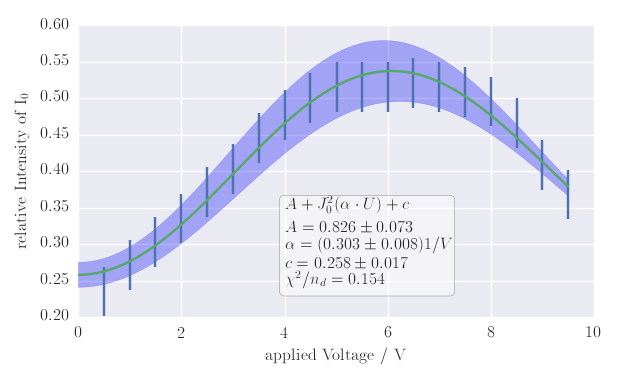
\includegraphics[width=1\textwidth]{analysis/figures/besselfit_001}
    \caption{
        The measurements and the least square fit with the maxima of first order, where
        the maxima were calculated with $I = (I_{\mathrm{left}} +  I_{\mathrm{right}})/2$.
        For further details on the applied procedure, see for figure~\ref{fig:besselfit_000}.
        Additionally we notice that the method estimating the maxima is encumbered by the 
        bad resolution of the peaks itself, such that they are not separated as they should. 
        Following from this we receive a huge systematic error, not being reflected in the
        statistical errors resulting from the least squares fit. \\
        $\Rightarrow$ The important characteristic value $\alpha$ disagrees 
        with the result of the maxima of zeroth order, which
        should in theory be the same. Noting that the $\chi^2$ test is lower then 1 (which would rather indicate that
        the given errors are too small or the hypothesis is wrong) we remark that the 
        systematic errors have an huge impact on the result, reflecting
        also in the disagreement within the parameters $A$ and $c$. 
        }
    \label{fig:besselfit_001}
\end{figure}


\begin{SCfigure}
    \caption{
        As before, only $A$ and $c$ are coupled, which is also visible in the
        bigger error. Since $\alpha$ is (according to the least squares fit)
        independent of the others, the systematic error described before (see caption of figure~\ref{fig:besselfit_001}) 
        cannot depend on the amplitude or a constant background noise alone, 
        but has to be related to the increased curvature
        visible in an higher $\alpha$.}
    \begin{tabular}{|r|r|r|r|}
        \hline 
        \cellcolor{tabcolor}&\cellcolor{tabcolor}$\alpha$&\cellcolor{tabcolor}$A$&\cellcolor{tabcolor}$c$\\ \hline 
        \cellcolor{tabcolor}$\alpha$&$0.00006$ &$-0.00004$ &$-0.00000$ \\ 
        \cellcolor{tabcolor}$A$&$-0.00004$ &$0.00532$ &$-0.00110$ \\ 
        \cellcolor{tabcolor}$c$&$-0.00000$ &$-0.00110$ &$0.00029$ \\ \hline \hline
        \cellcolor{tabcolor}$\alpha$&\multicolumn{3}{r|}{$0.30305 \pm 0.00792$ }\\ 
        \cellcolor{tabcolor}$A$&\multicolumn{3}{r|}{$0.82599 \pm 0.07293$ }\\ 
        \cellcolor{tabcolor}$c$&\multicolumn{3}{r|}{$0.25782 \pm 0.01709$ }\\ 
        \hline
    \end{tabular}
\end{SCfigure}
\newpage
\begin{figure}[htpb]
    \centering
    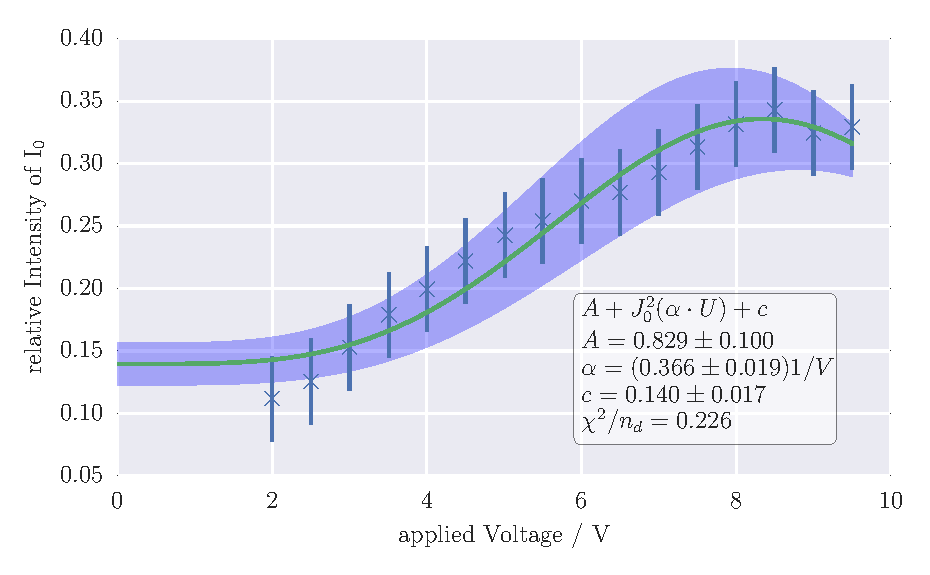
\includegraphics[width=1\textwidth]{analysis/figures/besselfit_002}
    \caption{This is the fit of the maxima of second order. For
    introductory remarks please see figure~\ref{fig:besselfit_000} and figure~\ref{fig:besselfit_001}.
    Again, as already observed in the maxima of first order, the curvature $\alpha$ has increased again.
    We want to emphasize the fact that the unreliability of this analysis is very low, because of \\
    \textbf{a) the low resolution} of the peaks such that they were not clearly separated 
    from the other maxima.\\
    \textbf{b) the strong disagreement} of $\alpha$ with the result of the other maxima, 
    further indicating to the systematic error.   
    }
    \label{fig:besselfit_002}
\end{figure}

\begin{SCfigure}
\caption{
    Since the fit is not reliable (as mentioned in figure~\ref{fig:besselfit_002}), 
    the covariance matrix along with the errors cannot have further significance.
    We note that the errors are too small to take into account the strong deviation to the
    other results. They should be corrected with an inherent systematic error, as considered in
    the remarks of figure~\ref{fig:besselfit_000} and figure~\ref{fig:besselfit_001}.
}
 \begin{tabular}{|r|r|r|r|}
 \hline 
\cellcolor{tabcolor}&\cellcolor{tabcolor}$\alpha$&\cellcolor{tabcolor}$A$&\cellcolor{tabcolor}$c$\\ \hline 
 \cellcolor{tabcolor}$\alpha$&$0.00037$ &$0.00028$ &$-0.00013$ \\ 
\cellcolor{tabcolor}$A$&$0.00028$ &$0.00992$ &$-0.00137$ \\ 
\cellcolor{tabcolor}$c$&$-0.00013$ &$-0.00137$ &$0.00029$ \\ \hline \hline
\cellcolor{tabcolor}$\alpha$&\multicolumn{3}{r|}{$0.36608 \pm 0.01934$ }\\ 
\cellcolor{tabcolor}$A$&\multicolumn{3}{r|}{$0.82888 \pm 0.09961$ }\\ 
\cellcolor{tabcolor}$c$&\multicolumn{3}{r|}{$0.13956 \pm 0.01695$ }\\ 
\hline
\end{tabular}
\end{SCfigure}
\newpage
\clearpage
\begin{figure}[htpb]
    \centering
    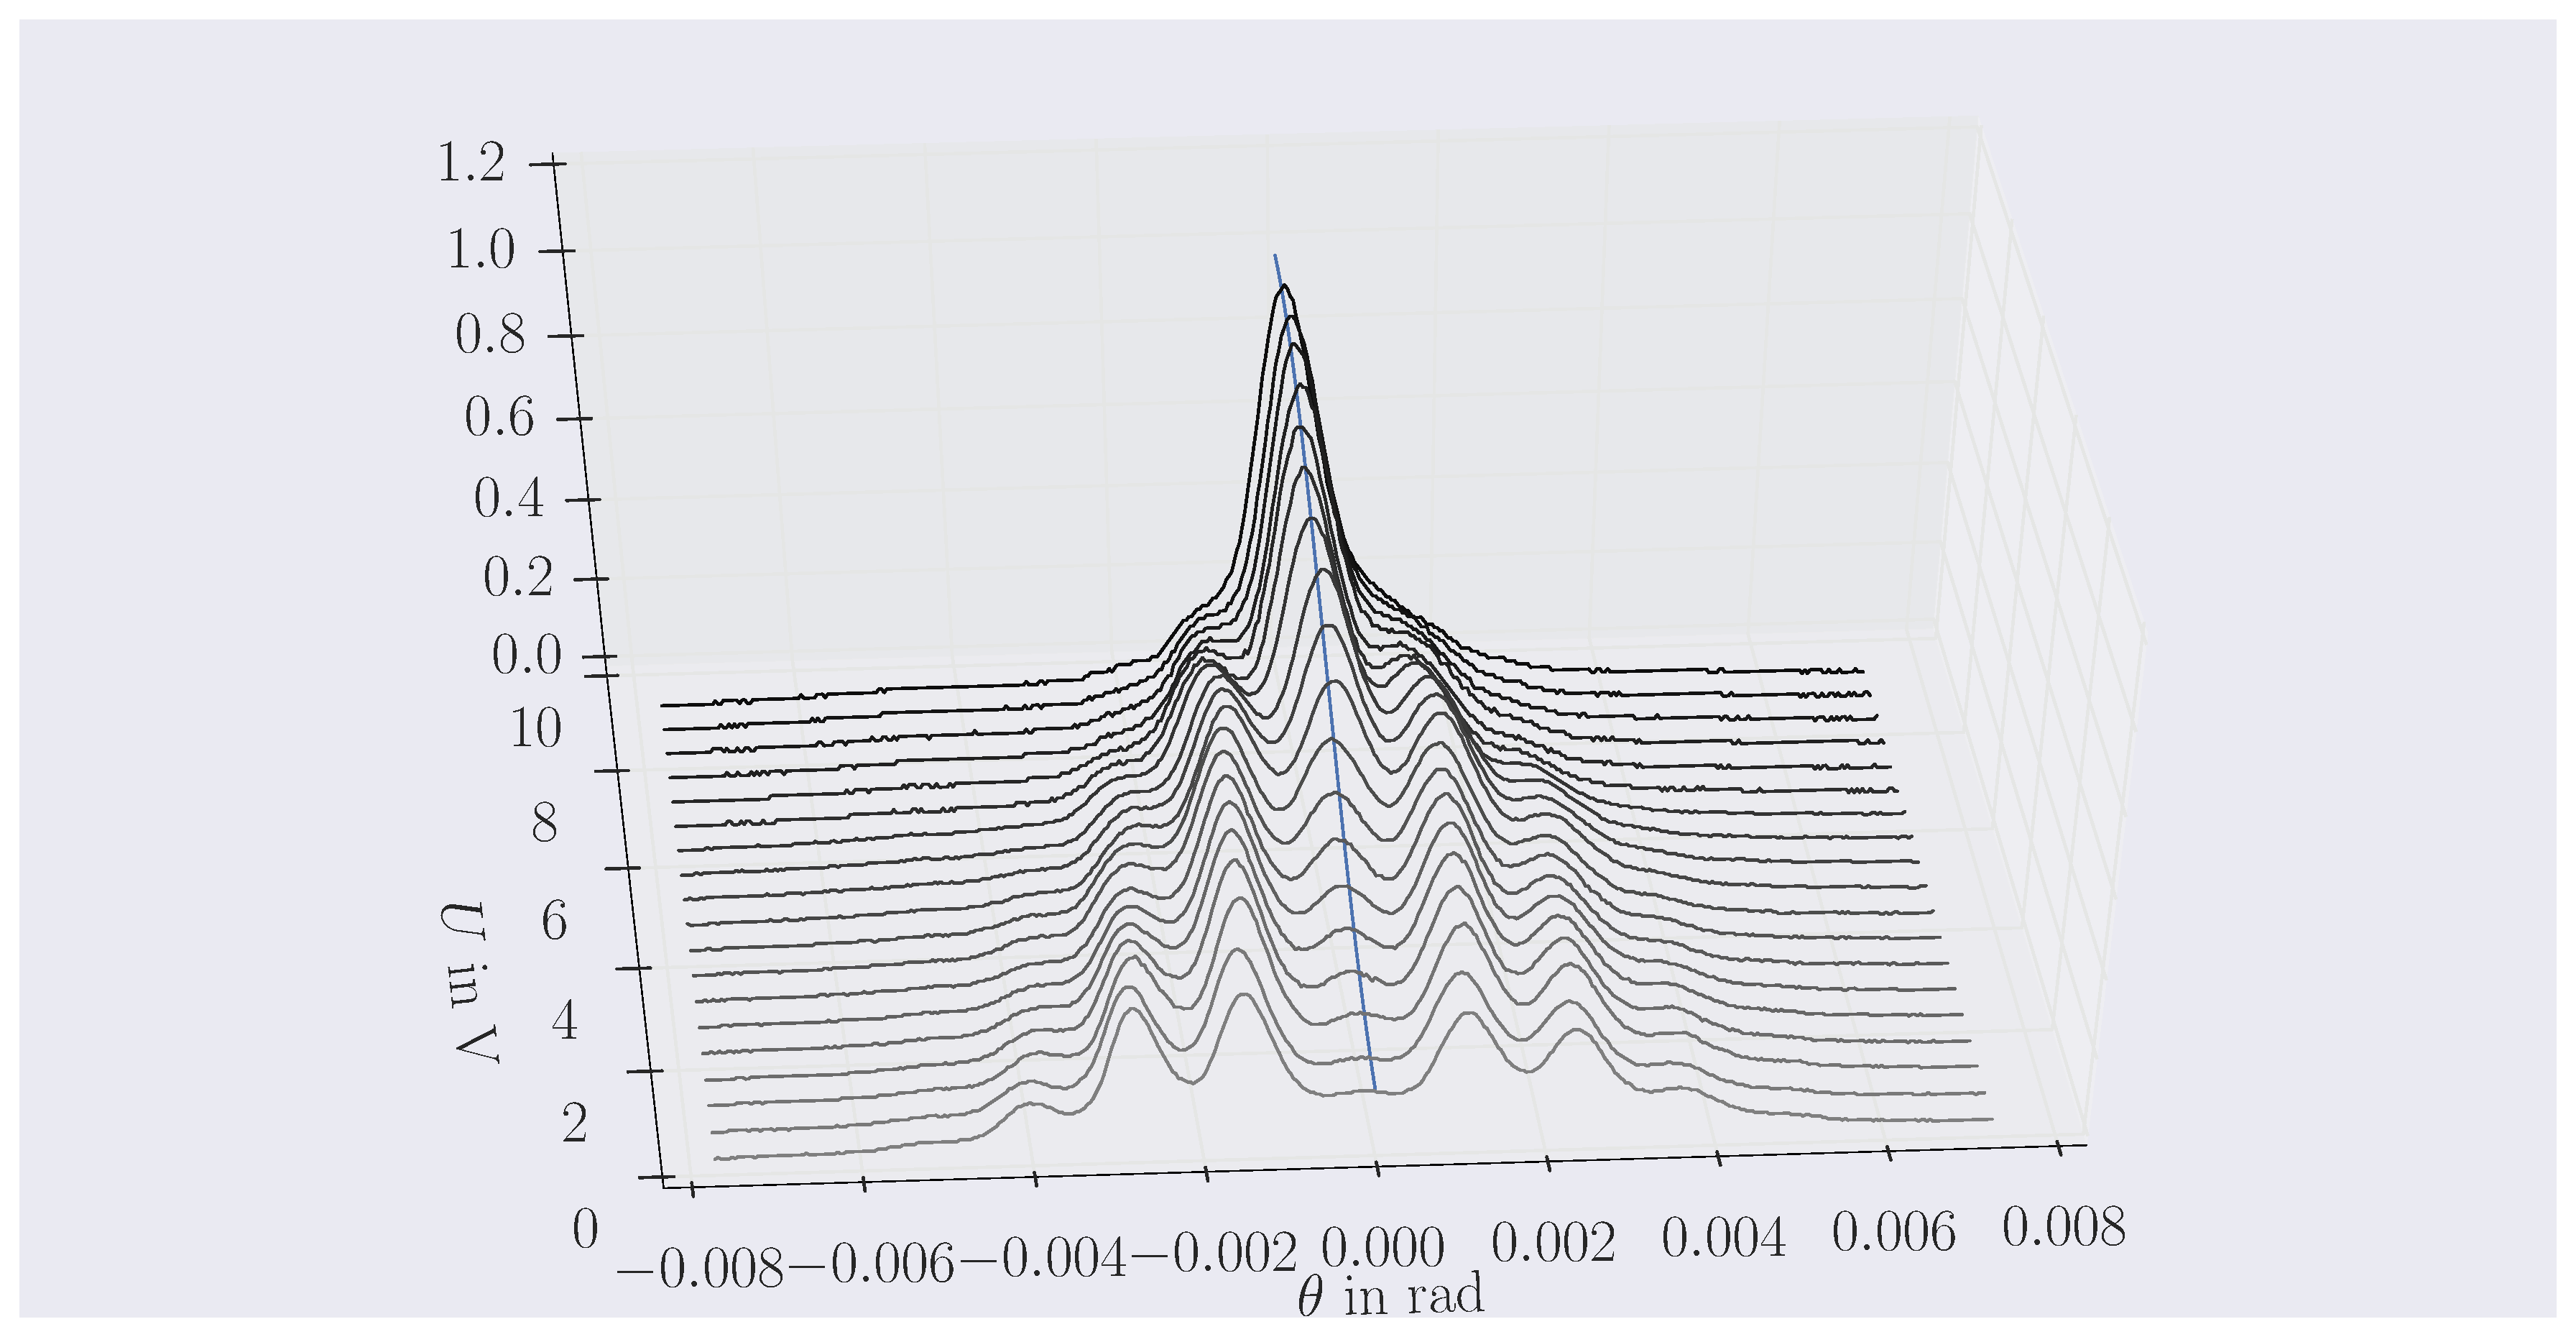
\includegraphics[width=1\textwidth]{./figures/plot3d}
    \caption{   Visualization of the measurements with 3d projection.
    }
    \label{fig:plot3d}
\end{figure}


\subsubsection{Sonic wave length}
As far as we can consider the results of our measurements,
we can estimate the sonic wave length with the already
given equation 
\begin{equation}
\sin(\theta_m) = \frac{m \lambda}{\Lambda}.
\end{equation}
We notice that the estimated value is not constant for all voltages, unlike as predicted by theory; 
see figure~\ref{fig:soundspeed} for the discrepancy of estimating $\Lambda$ with the maxima 
of first order for different $U$.
We suspect this to be due mostly to the described shortcomings in resolution. 
However, we note other systematical errors might be induced by other 
electro-optical effects such as dispersion. The instability of frequency generation
seems to be of negligible order.
\begin{figure}[H]
    \centering
    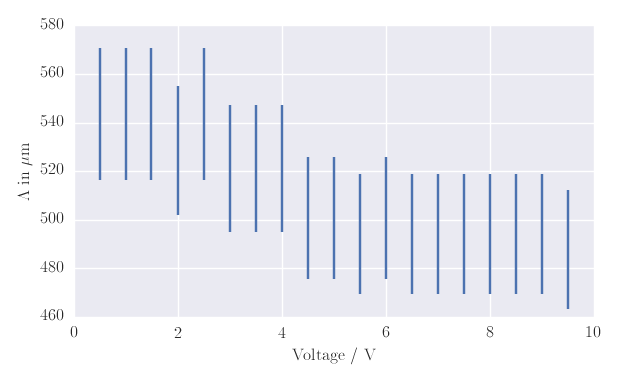
\includegraphics[width=1\textwidth]{analysis/figures/soundspeed}
    \caption{
        These are the estimated values for $\Lambda$ with regards to the maxima of first order.
        We notice that the wavelength is not constant for all voltages. The error bar is given by
        gaussian error propagation of the uncertainty in finding the position of the maxima (the
        width of the maximum).}
    \label{fig:soundspeed}
\end{figure}
The mean value of the values for maxima of first order yields
\begin{equation}
    \Lambda = \left [511 \pm 26 \right ]\, \mu\mathrm{m}.
\end{equation}
In order to judge the quality of this estimation we can alternatively calculate the
wavelength with the sonic speed in Isooctane $c = 1111\,$m/s (given in \cite{staatsexamen})
and the 
frequency of the piezoelectric crystal $f =2132 \pm 5\,$Hz (where the uncertainty is given
by the unstable signal we measured over the whole experiment):
\begin{equation}
\Lambda = \frac{c}{f} = \left [521 \pm 1 \right ] \mu m
\end{equation}
Despite all difficulties discussed before, our prior estimation 
lies in this more precise value within the stated error. 
We thus conclude that at least for the first maximum, 
the obtained data can be used for the calculation. 
This further underlines the agreement of Raman-Nath theory
with the observations.
which is within the range of our former estimation. 

